\chapter{Terminología DevOps}\label{ch:devops}
%************************************************
Al haber consolidado la metodología de desarrollo SCRUM en los capítulos anteriores (\ref{sec:metodologia}), sabemos que dicha metodología pertenece a un ámbito de desarrollo iterativo e incremental, donde el proyecto se planifica en diversos bloques temporales. Debido a esto es muy frecuente que el equipo de desarrollo tenga numerosas entregas, ya que debe proporcionar una versión incrementada en cada iteración, esto también se suele denominar como despliegue.

\vspace{0.3cm}

Generalmente para proporcionar un despliegue el equipo de desarrollo se divide en dos ámbitos o departamentos. El primero tiene la función de desarrollo o la propia codificación de la aplicación, reconocido como «development» o «Dev» del inglés. El segundo se encarga de la parte operacional o el gestionado de versiones y la parte física del despliegue, reconocido también como «operations» o «Ops». \cite{redahat-devops}

\vspace{0.3cm}

El problema más usual es que ambos departamentos tienden a estar separados, por lo que el flujo de comunicación tiende a fallar y a tener retrasos a la hora de proporcionar el despliegue. Bajo esta premisa, surge una solución en 2009 denominada como \textit{DevOps}, la cual tiene como propósito unificar estos dos ámbitos \cite{redahat-devops}

\vspace{0.3cm}

\begin{figure}[H]
    \centering
    \myfloatalign
    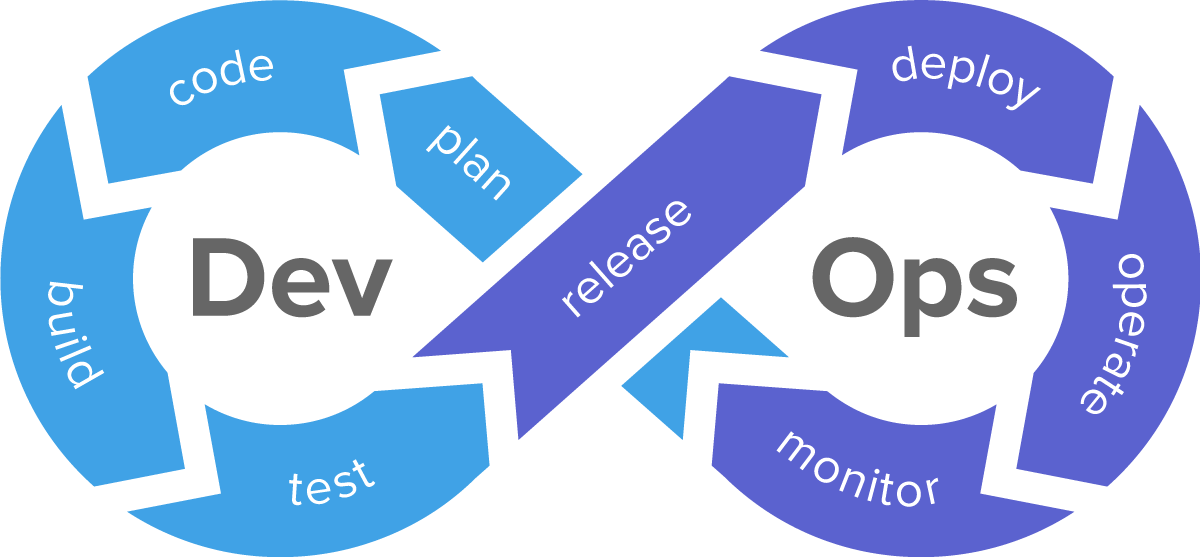
\includegraphics[width=0.7\textwidth]{gfx/devops-explicativo.png}
    \caption[Imagen explicativa del concepto DevOps]{Imagen explicativa del concepto DevOps \cite{azure-devops}.}\label{gfx:devops-explicativo}
\end{figure}

En resumen, \textit{DevOps} trata de romper estos silos organizativos establecidos y intenta centrarse en la mejora de calidad de la entrega al cliente. Para ello, \textit{DevOps} se apoya en tres principios o también llamadas «the three ways», las cuales se deben implementar de forma consecutiva. \cite{ilimit-devops}

\begin{enumerate}
    \item\textit{Mejora del flujo de entrega}: consiste en general valor al producto, mediante entregas del software de una forma temprana y periódica. Tratando de dividir los procesos en tareas más pequeñas o automatizando todas las tareas que sean posibles, con esto se consigue un aumento del flujo de trabajo global, ya que en este caso un proceso no ralentiza a otro. \\
    Un ejemplo de este principio puede ser la ejecución de tests u otras operaciones cada vez que haya cambios en el repositorio del código fuente.
    \item\textit{Buen uso de los ciclos de feedback}: consiste en el uso de la retroalimentación con el objetivo de optimizar los procesos, es decir, cada vez que se lleve a cabo una entrega conviene tener un \textit{feedback} rápido y constante. Con esto se que consigue que los ciclos de retroalimentación obtengan las información necesaria para que las correcciones se puedan aplicar de manera continua. \\
    Un ejemplo de ello puede ser la monitorización del sistema y la comunicación ante la detección de errores.
    \item\textit{Asentar el aprendizaje y la mejora continua}: se centra en aplicar todo lo anteriormente realizado y aprendido para implementar un sistema de mejora continua. De esta manera se consigue innovar el producto pero sin criminalizar los errores mediante el aprendizaje y las pruebas continuas. \\
    Un ejemplo puede llegar a ser usar programas extremos de pruebas o prestaciones.
\end{enumerate}

\subsection{Implementación Back-end}

Explicar Poetry, mypy, flake8 y pytest + esquema CI

\subsection{Implementación Front-end}